64. \begin{figure}[ht!]
\center{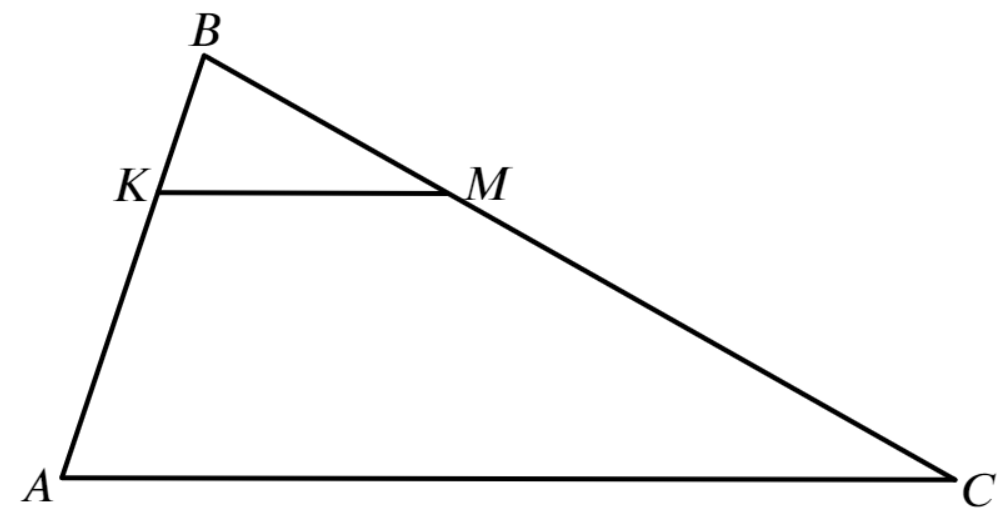
\includegraphics[scale=0.35]{g9-63.png}}
\end{figure}\\
Пусть $BK=3x,$ тогда $KA=4x,\ AB=7x.$ Треугольники $ABC$ и $KBM$ подобны по двум углам (соответственные $BAC$ с $BKM$ и $BCA$ с $BMK$), значит $\cfrac{AC}{KM}=\cfrac{AB}{BK},\ \cfrac{AC}{18}=\cfrac{7x}{3x},\ AC=42$см.\\
